\documentclass[11pt]{article}

\usepackage{amsmath}
\usepackage{amssymb}
\usepackage[utf8]{inputenc}
%\usepackage[latin1]{inputenc}
\usepackage[spanish]{babel}
\usepackage[left=3cm,right=3cm,top=3cm,bottom=2.5cm]{geometry}
\usepackage{amsmath,amssymb,latexsym,color,graphicx,verbatim}
\usepackage{mathrsfs}
\usepackage{layout}
\usepackage{graphicx}
\usepackage{multirow}
\usepackage[table,xcdraw]{xcolor}
%COLOCA COMANDOS EN ESPAÑOL
%\renewcommand{\contentsname}{Contenido}
%\renewcommand{\partname}{Parte}
%\renewcommand{\appendixname}{Apéndice}
%\renewcommand{\figurename}{Figura}
%\renewcommand{\tablename}{Tabla}
%\renewcommand{\abstractname}{Resumen}
%\renewcommand{\refname}{Bibliografía}
%FIN DEL BLOQUE
\usepackage[acronym,shortcuts]{glossaries} %PARA UN GLOSARIO DE ACRÓNIMOS
\makeglossaries
\usepackage[font=small]{caption}
\usepackage[colorlinks = true,
                     linkcolor = blue,
                     citecolor = red,
                     urlcolor = blue]{hyperref}

\baselineskip0.75cm
\parskip0.5cm
\parindent0cm

\begin{document}


\begin{titlepage}
\centering \textbf{{\Large {\sc Estudio del último eclipse cromosférico de $\zeta$  Aurigae, otoño 2019}}}

\vfill
\centering {\Large Propuesta de trabajo de grado para optar al t\'itulo de F\'isica}
\vfill
\hfill

\centering {\textbf{\Large Natalia Lucía Oliveros Gómez$^{1,2}$}}

\vfill

\centering {\Large Director: Ph.D Klaus-Peter Schröder $^{3}$}

\centering {\Large  Co-Director: Ph.D Luis Alberto Núñez$^{1,2}$}

\centering {\Large  Co-Director: M.Sc Faiber Danilo Rosas$^{3}$}


\hfill




{{\Large $^1$Grupo de Investigaci\'on en Relatividad y Gravitaci\'on GIRG}} \\
{{\Large$^2$Grupo Halley de Astronom\'ia y Ciencias Aeroespaciales}} \\
{{\Large$^3$Grupo de Investigación en Física Estelar, Universidad de Guanajuato}} \\

\vfill
\vfill

\centering {\Large Universidad Industrial de Santander\\Facultad de
Ciencias\\Escuela de F\'{i}sica\\Bucaramanga\\2020}


\end{titlepage}


\newpage

\tableofcontents

%\newpage

%\acrodef{LAGO}{Latin American Giant Observatory}

\newpage




%%%%%%%%%%%%%%%%%%%%%%%%%%%%%%%%%%%%%%%%%%%%%%%%%%%%%%%%%%%%%%%%%%%%%%%%%%%%%%%%%%%%%%%%%%%%%%

\begin{table}[htbp]
\begin{center}
\resizebox{14cm}{!}{
\begin{tabular}{|l|l|l|l|l|}
\hline
\multicolumn{5}{|l|}{\begin{tabular}[c]{@{}l@{}}\textbf{Título de la propuesta:}\\ Estudio del último eclipse cromosférico de $\zeta$ Aurigae, otoño 2019\end{tabular}}           \\ \hline
\multicolumn{5}{|l|}{\begin{tabular}[c]{@{}l@{}}\textbf{Nombre del estudiante:}\\ Natalia Lucía Oliveros Gómez\end{tabular}}                                                    \\ \hline
\textbf{Código:} 2160778                          & \multicolumn{3}{l|}{\textbf{E-mail:} onatalialucia@gmail.com}                              & \textbf{Cel:} 3123154756                         \\ \hline
\multicolumn{5}{|l|}{\begin{tabular}[c]{@{}l@{}}\textbf{Nombre del grupo de Investigación:}\\ Física Estelar de la Universidad de Guanajuato\end{tabular}}                                           \\ \hline
\multicolumn{5}{|l|}{\begin{tabular}[c]{@{}l@{}}{\textbf{Dirección:} Callejón de Jalisco S/N, Col. Valenciana , CP: 36023\\ Guanajuato, Gto, México. Departamento de Astronomía}                 \end{tabular}}                                                                            \\ \hline
\textbf{Tel:} 1 473 732 0006                                     & \multicolumn{4}{l|}{\textbf{E-mail: } astrokp85@gmail.com}                                                                                                \\ \hline
\multicolumn{5}{|l|}{\begin{tabular}[c]{@{}l@{}}
{\textbf{Líneas de investigación desarrolladas por el grupo:} Atmósferas estelares,\\ evolución estelar, sistemas binarios }\end{tabular}}              \\ \hline
\multicolumn{5}{|l|}{\begin{tabular}[c]{@{}l@{}}\textbf{Profesor de la Escuela de Física que dirigirá el trabajo:}\\ Ph.D Luis Alberto Núñez de Villavicencio Martínez \end{tabular}} \\ \hline
\multicolumn{5}{|l|}{\begin{tabular}[c]{@{}l@{}}\textbf{Profesional del grupo de investigación que servirá de tutor:}\\ Ph.D Klaus-Peter Schröder\end{tabular}}              \\ \hline
\end{tabular}}
\end{center}
\end{table}

\newpage
%%%%%%%%%%%%%%%%%%%%%%%%%%%%%%%%%%%%%%%%%%%%%%%%%%%%%%%%%%%%%%%%%%%%%%%%%%%%%%%%%%%%%%%%%%%%%%
\begin{abstract}
En este proyecto se realiza un análisis de la variación de la densidad de masa columnar en la crómosfera de la estrella $\zeta$ Aurigae durante su último eclipse en otoño de 2019. Se hace un estudio de la variabilidad temporal de la línea K de CaII (3934 A), usando espectros de alta S/N y buena resolución ~20000 obtenidos por TIGRE-HEROS. Usando datos de eclipses anteriores para el mismo sistema, se propone un modelo que explique el cambio de densidad de masa columnar con la altura en la cromósfera de ésta estrella y la dinámica del sistema.

\vspace{0.5cm}
\textbf{Palabras clave:} Estrellas binarias eclipsantes, cromosfera estelar, curvas de crecimiento, espectroscopia.

\end{abstract}


\begin{figure}
  \centering

  \label{Figura 1}
\end{figure}


\section{Grupo de Investigación de la Universidad de Guanajuato}

El grupo de investigación de \textit{Física Estelar}, al cual pertenece el Ph.D Klaus-Peter Schröder y el MSc. Faiber Rosas tiene como objetivo el estudio del nacimiento, la evolución y la muerte de las estrellas frías y las estrellas masivas.  Este grupo de investigación aplica los principios de la física para modelar el interior de la estrella, su atmósfera y su viento, así como las interacciones en sistemas estelares binarios y en sistemas planetarios. Se aplican modelos teóricos así como datos observacionales del telescopio TIGRE  \footnote{El telescopio TIGRE, por sus siglas Telescopio Internacional Guanajuato Robótico Espectroscópico el cual antes era llamado HRT (por sus siglas, Hamburgo Robotic Telescope), es una de las herramientas por las cuales se tiene una un convenio bilateral entre la Universidad de Guanajuato - México, la Universidad de Hamburgo - Alemania y la Universidad de Liège - Bélgica.} \cite{schmitt2014tigre}, para el análisis de propiedades intrínsecas de estrellas frías.

\noindent De manera mas especifica, para estrellas masivas, la investigación se centra en la estructura de los vientos estelares, modelar efectos de rotación,  inestabilidades intrínsecas, interacciones en sistemas binarios y  evolución estelar. Se busca determinar con buena precisión parámetros principales como temperatura efectiva, gravedad superficial y composición química, con el uso de modelos fotosféricos generados con el código PHOENIX \cite{hauschildt2005cool} \footnote{Un código que permite modelar atmósferas estelares y espectros teóricos de diferentes tipos de estrellas.} y análisis de espectros del telescopio TIGRE. Lo cual permite comprender mejor la actividad y evolución de estrellas como el Sol. Para el caso de estrellas jóvenes, la investigación se centra en el cálculo de la emisión de polvo en sistemas circumplanetarios que las rodean; ésto nos permite caracterizar la distribución de material en estos discos, que a su vez tiene que ver con la presencia de planetas. 

\section{Lugar dentro de los proyectos del grupo de investigación}
\noindent Este proyecto se realizará en el marco de pasantía de investigación y está enfocado en el área de atmósferas estelares e interacción de sistemas estelares binarios. Se realizará el análisis de la cromosfera de un sistema binario con el uso de espectros tomados por el telescopio TIGRE ubicado en Guanajuato, México y códigos que permitan modelar atmósferas, uno de estos es PHOENIX; También se tendrán en cuenta parámetros principales que necesitan alta precisión como: temperatura efectiva, gravedad superficial y composición química. Este trabajo al estar bajo la dirección de del profesor Klaus-Peter Schröder, tiene un enfoque en evolución estelar y atmósferas estelares, más específicamente estudio de la cromósfera del sistema binario Zeta Aurigae en, el cual él analizó en los años 80 \cite{kps9}, \cite{kps1O}. Por lo tanto, con la experiencia en este sistema, resulta interesante retomar estas investigaciones ya que en la actualidad se tienen mejores tecnologías que en aquella época, lo cual permite desarrollar mejores análisis.

\section{Problema de investigación}

\noindent Los sistemas de estrellas binarias eclipsantes están formados por dos estrellas cuyo plano orbital está orientado hacía la Tierra, es decir, podemos observar los eclipses de estas estrellas. Por lo tanto, cuando se miden espectros de estos sistemas, en el transcurso del eclipse las componentes espectrales de cada estrella se superponen, haciendo que los espectros individuales no puedan ser reconocibles. Sin embargo, se puede hacer una sustracción de los espectros para cada estrella si se tienen espectros de la estrella principal sin eclipsar y así comparar con los espectros durante el eclipse. Cuando se logra la separación de espectros, este tipo de sistemas binarios son unas de las herramientas que tienen los astrónomos para obtener información de cantidades físicas fundamentales de las estrellas, como radios estelares, velocidades orbitales, masas de manera muy precisa, consideraciones geométricas del eclipse y temperaturas efectivas \cite{schroder2009stars}.


\noindent En el transcurso del tiempo se han hecho análisis de sistemas binarios eclipsantes, en especial donde una de las componentes estelares es una estrella gigante fría, ya que estas normalmente se encuentran en su fase de gigante roja y son fáciles de reconocer. Además estas estrellas nos permiten obtener información que permita conocer de manera más clara los fenómenos físicos que ocurren en la cromosfera de las estrellas. Cuando la estrella compañera se aproxima a la estrella gigante roja, en los espectros se pueden apreciar líneas de absorción adicionales que revelan cambios en temperatura, densidad, extensión y movimiento de la cromosfera, que es la región estelar de transición turbulenta entre la fotosfera (superficie de la estrella) y la corona (donde se transporta y pierde materia por vientos solares). Dichos cambios apreciados en el espectro se deben a la presencia del eclipse y estos datos tiene alta relevancia en la física estelar ya que con los sistemas binarios se obtiene una forma de medir la masa estelar directamente con el uso de las leyes de Kepler y al conocer las masas con precisión sirven para calibrar trayectorias estelares evolutivas.

\noindent El sistema binario a analizar en este proyecto es Zeta Aurigae, el cual está compuesto por $\zeta$ Aur A, una supergigante roja de tipo espectral K5II; y $\zeta$ Aur B una estrella de la secuencia principal de tipo espectral B7V \cite{shenavrin2011vizier}. Éste sistema se encuentra ubicado en la constelación de Auriga, el cual tiene un plano orbital que coincide con la línea de visión terrestre, y en él se presenta el fenómeno de eclipses atmosféricos, los cuales se pueden observar a simple vista, ya que durante los eclipses la la magnitud de $\zeta$ Aur A disminuye a +3,99 en la banda V. Este sistema resulta relevante, ya que hasta el momento no ha sido muy analizado y no se tienen muchos datos observacionales del mismo.
\vspace{2mm}

\noindent En trabajos anteriores se han hecho análisis de fotometría y espectroscopia de este sistema con el enfoque de observar el cambio de las líneas de absorción durante el eclipse, dando información relevante respecto a la geometría del eclipse, velocidades radiales, masa estelar y luminosidad \cite{kps9}. También se han hecho análisis a partir de \textit{curvas de crecimiento experimentales} \cite{complete}, las cuales son gráficos del ancho equivalente de la línea ($log(W_{\lambda})$) se relaciona con la profundidad de la línea en el espectro ($log(\tau)$) que se refiere a la fuerza de la línea en el espectro. Estas curvas se hacen teniendo en cuenta modelos de densidad e intentando analizar la estructura cromosférica partiendo de la ionización, turbulencia y cambios en la temperatura efectiva. Sin embargo, aún no hay conclusiones específicas de lo que pasa en la atmósfera estelar respecto al cambio en la densidad de átomos del elemento analizado en la fotosfera y cromosfera a medida que cambia la altura, es decir, cambio en la densidad de átomos de H por área por camino óptico entre la estrella y el observador \cite{rybicki2008radiative}. Inicialmente en los espectros se observaba que todas las líneas metálicas tienen el mismo comportamiento, es decir, que la ionización no cambia con respecto a la altura de la atmósfera, donde para bajas alturas la ionización de los metales es casi completa. Pero en el caso de  las líneas de absorción de H y Ca II K (que son las líneas más afectadas durante los eclipses) cambia la ionización media rápidamente con la altura en un factor de 100 con respecto a los demás metales, es decir, que las líneas de Ca II K son un caso anómalo en los eclipses y no se conoce la razón física de que esto suceda \cite{complete}.

\noindent De acuerdo a los trabajos citados anteriormente, surge la necesidad de hacer un análisis que verifique lo que se ha analizado hace más de 30 años, desde un  enfoque espectroscópico de la densidad de columna cromosférica, la cual tiene una dependencia con la altitud del eclipse. De esta forma intentar aclarar fenómenos que antes no podían ser explicados con los modelos de la época según las observaciones espectroscópicas, como por ejemplo la dinámica envuelta en la cromosfera por medio de perfiles de densidad. 

\noindent Es muy importante en este planteamiento la importancia del uso de espectroscopia ya que las líneas de absorción varían con la densidad. En la parte alta se observan algunas líneas fuertes y en la parte baja de la atmósfera hay muchas líneas débiles. En el caso de espectros puros se pueden medir mientras no esté eclipsado, con las líneas H y K de Ca II (396,847 nm y 393,368 nm) de la fotosfera que son bastante anchas y se comprueba la emisión central de la estrella gigante, estas líneas estándar tienen características de tipo tardío, ya que es una estrella K y se puede definir una escala $\lambda$. También se pueden medir mediante perfiles de dispersión. Para los espectros compuestos, es decir durante el eclipse, se observan cambios en el espectro, estos son de dispersión media y se observan como ``ruido'' en la contribución al espectro puro de la gigante donde las líneas K desvanecen y se observa que por la presencia de la estrella B7 se tienen líneas anchas e intensas de Ca II que cambian su ancho y fuerza durante el eclipse y no es fácil de hacer una distinción de componentes estelares; además no es posible saber cómo hacer la sustracción de espectros para obtener el de la estrella B. En el eclipse total hay una fuerte absorción mayor de Ca II K y por ende más cantidad de líneas de absorción cromosférica, y es la oportunidad de hacer la sustracción de los espectros de la gigante para hacer las respectivas curvas de crecimiento experimentales. 



%%%%%%%%%%%%%%%%%%%%%%%%%%%%%%%%%%%%%%%%%%%%%%%%%%%%%%%%%%%%%%%%%%%%%%%%%%%%%%%%%%%%%%%%%%%%%%
\section{Justificación}
%Por lo que el análisis de este tipo de estrellas resulta muy interesante y un escenario aplicable para conceptos físicos que se han aprendido durante la carrera de 

\vspace{3mm}
Dos de las características más relevantes para analizar un sistema de estrellas binario es que éste sea brillante, para que sea fácil de detectar con telescopios y además que tenga un periodo de orbita corto, de tal manera se podrá analizar mayor cantidad de veces y se tienen mejores resultados. En el caso de nuestro sistema a analizar, Zeta Aurigae es bastante brillante, sin embargo no basta con esto, ya que su periodo orbital es grande (972 días), por lo que éste no ha sido muy analizado, salvo con algunas observaciones que se dieron del sistema pero hace aproximadamente 30 años, por lo que resulta importante retomar o tener en cuenta algunos de los resultados que se han obtenido y verificarlos para presentar mejoras o aportes a algunos desarrollos respecto a este sistema binario, como en el caso de la densidad columnar y que efectos tienen los cambios de esta en el proceso del eclipse.

En \cite{kps1O} se tiene un enfoque sobre la cromosfera en el que se ha considerado una ley de potencias de forma exponencial (ley barométrica exponencial) que relaciona las escalas de densidad de columna y altura. Para el caso de alturas pequeñas en la fotosfera la densidad columnar se podía considerar constante (tomando un promedio) ya que aunque tenía un crecimiento, éste era muy lento y por lo tanto se podía despreciar, la cual se expresa en la ecuación (\ref{eq:leybaro}). Sin embargo, en espectros actuales del eclipse de otoño del 2019 con mejor resolución espectral $\sim 20000$ y buena relación S/N 200-300 se observa que las variaciones de la densidad de columna puede no estar siguiendo el mismo modelo que se había considerado, ya que los cambios que se estaban considerando como constantes, pueden realmente afectar posibles conclusiones de la dinámica de la cromosfera de las estrellas. Puede ser necesario considerar otro modelo de densidad que se ajuste mejor a los parámetros geométricos del eclipse y que tenga en cuenta dichas variaciones como el caso de ionización de elementos en la atmósfera, reduciendo así las incertidumbres.

\begin{equation}
    n(h) = n_o \exp{(-h/\alpha)}
    \label{eq:leybaro}
\end{equation}
\vspace{2mm}

Gracias a las nuevas observaciones realizadas por TIGRE, con estos datos se puede analizar y conocer la dinámica del sistema como lo son la geometría del eclipse, masa estelar, luminosidad, velocidad radial, temperatura efectiva y densidad de columna, los cuales están englobados al hacer un análisis de la cromosfera de la estrella gigante pura con respecto a las variaciones de la misma en el transcurso del eclipse.

En el siglo pasado, se consideraba que la astronomía tenía un carácter de una ciencia puramente observacional y empírica, sin embargo en la actualidad, se ha confirmado que no basta solo con modelos empíricos, sino que es necesario que estos estén sustentados física y matemáticamente, por lo tanto es lo que ahora se ha convertido en ``Astrofísica'': la aplicación de la física a los objetos astronómicos. En este sentido, utilizamos el universo como un enorme laboratorio natural, en el que podemos probar nuestras teorías físicas en condiciones extremas (temperaturas altas o bajas, densidades, presiones), que no podemos realizar y probar en laboratorios artificiales. De esta manera, la astronomía y la astrofísica se ha convertido en un campo muy importante de la física.

Por lo tanto, para realizar el análisis cromosférico de este sistema binario es imprescindible aplicar conceptos físicos aprendidos en los cursos de la Universidad Industrial de Santander, como espectroscopia donde es muy relevante conocer la importancia de la interacción fotón-átomo que incluye tipos de absorción, dispersión de resonancia, emisión (re-emisión); también muy relevante teoría de radiación, como la transferencia radiativa que es muy importante al observar qué pasa con la radiación al pasar por la atmósfera de una estrella; cabe resaltar también que es importante en cuanto a teoría atómica que los átomos están cambiando por todos los procesos llevado a cabo en la estrella (por procesos de ionización y demás). Por último es importante recordar que en este caso para el sistema de Zeta Aurigae no resultan relevantes los efectos relativistas ya que no se trata de un sistema binario en el que las estrellas estén muy próximas (4,2 UA) y estén interactuando más allá de la gravitación que las mantiene en órbita, no está cambiando la métrica ni otros aspectos en lo que la perturbación relativista sea relevante, por lo tanto se analiza la dinámica de este sistema como un problema clásico.

\noindent Adicionalmente debido a mi aspiración de hacer una maestría en astronomía es muy relevante el tener la oportunidad de trabajar con datos reales de un observatorio astronómico internacional y datos del repositorio de Gaia de la ESA que son los datos de paralaje con mayor precisión actualmente, que permiten calcular luminosidades estelares muy acertadas, y para hacer el análisis de estos datos es necesario tener hacer consideraciones relevantes y aplicar modelos físicos para reducir datos y comprender la física que se encuentra en ellos con el enfoque astronómico de la rama estelar.

%%%%%%%%%%%%%%%%%%%%%%%%%%%%%%%%%%%%%%%%%%%%%%%%%%%%%%%%%%%%%%%%%%%%%%%%%%%%%%%%%%%%%%%%%%%%%%
\section{Objetivos}

%%%%%%%%%%%%%%%%%%%%%%%%%%%%%%%%%%%%%%%%%%%%%%%%%%%%%%%%%%%%%%%%%%%%%%%%%%%%%%%%%%%%%%%%%%%%%
\textbf{Objetivo General}

\begin{itemize}
\item Comparar la absorción cromosférica y el cambio de la densidad de columna N(h) del eclipse de otoño 2019 con un antiguo eclipse de 1987.
\end{itemize}
\textbf{Objetivos Espec\'ificos}
\begin{enumerate}
    \item Cuantificar el ancho equivalente las líneas claves (Ca II) de las dos estrellas y la  absorción cromosférica

    \item Realizar un análisis de las curvas de crecimiento observacionales

    \item Deducir la densidad en columna y comparar con los resultados publicados, obtenidos en eclipses pasados
\end{enumerate}

%%%%%%%%%%%%%%%%%%%%%%%%%%%%%%%%%%%%%%%%%%%%%%%%%%%%%%%%%%%%%%%%%%%%%%%%%%%%%%%%%%%%%%%%%%%%%%

\section{Metodolog\'ia}

Para alcanzar el objetivo general, es necesario culminar con los objetivos específicos, por los tanto  se proponen una serie de actividades que están relacionadas con cada uno de los objetivos específicos de acuerdo al número asignado anteriormente:

\begin{itemize}

\item[1.1] Instalar y aprender a usar softwares para análisis de espectros:
\begin{itemize}
    \item iSpec: Genera síntesis espectrales, permite encontrar parámetros estelares mediante ajuste de líneas espectrales y ajuste del continuo usando modelos \cite{blanco2014determining}, \cite{blanco2019modern}.
    \item Código que permite analizar la absorción de la línea K de Ca II, permite medir el ancho de línea y el área bajo la curva
    \item Código de evolución estelar: Genera trayectorias evolutivas para determinar masas y edades de las estrellas en un diagrama HR \cite{pols1998stellar}, \cite{schroder1997critical}.
\end{itemize}
\item[1.2] Clasificar la lineas cromosféricas de la estrella gigante y la secundaria
\item[1.3] Obtener un registro de los espectros en orden temporal y calcular en cada caso la altitud proyectada de la compañera sobre la fotosfera del gigante

\item[1.4]  Usar el espectro puro de la gigante durante la totalidad del eclipse para sustraer los espectros compuestos para obtener y obtener el espectro puro la compañera, en el cual se vean las lineas cromosféricas

\item[1.5] Cuantificar el ancho equivalente de las líneas cromosféricas (área de línea de absorción dividido por el continuo local)

\item[2.1] Graficar curvas de crecimiento para cada sesión del eclipse (estrella individual parcial `tanto entrada como salida' y total). Igualmente para el hidrógeno y para el Ca II 

\item[3.1] Comparar diferentes parámetros (\textit{ionización, temperaturas efectiva, ancho doppler,número de átomos, velocidades radiales}) con la densidades de columna N(h)

\item[3.2] Deducir un sencillo modelo de la densidad de columna en cada caso

 %%%%%%%%%%%%%%%%%%%%%%%%%%%%%%%%%%%%%%%%%%%%%%%%%%%%%%%%%%%%%%%%%%%%%%%%%%%%%%%%%%%%%%%%%%%%%%
\end{itemize}
\begin{comment}
Con estas actividades voy a poder desarrollar ciertas competencias que resultan muy útiles e importantes para trabajos a futuro:

\begin{itemize}
    \item Identificación de líneas espectrales y clasificación de espectros
    \item Uso de gráficas basado en plataformas de linux
    \item Entender y aplicar la física espectroscopia de líneas de absorción
    \item Obtener un fondo de la física de atmósferas estelares
\end{itemize}
\end{comment}


\section{Resultados esperados}

El resultado principal que se espera de este proyecto es encontrar cuáles son las diferencias y/o similitudes que hay entre los análisis que se han hecho del sistema Zeta Aurigae de hace 30 años con relación a los datos obtenidos del eclipse de otoño del 2019. Teniendo argumentos desde la ciencia respecto a qué se pueden deber los cambios que se puedan confirmar con respecto a estudios anteriores, teniendo en cuenta que la tecnología desde esa época a la actualidad ha cambiado y las herramientas que se tienen actualmente pueden ser más eficientes en aspectos técnicos.

Cabe resaltar que a medida que ha pasado el tiempo desde los análisis anteriores a la actualidad (aproximadamente 30 años) no ha pasado el tiempo suficiente como para que exista la posibilidad de que hallan cambios debido a la evolución estelar del sistema binario que puedan afectar de manera significativa los resultados obtenidos, por lo tanto sabremos que las condiciones en las que se analizaran son aproximadamente las mismas como para concluir que si hay cambios, estos se han efectuado bajo los mismos parámetros que se habían analizado antes.

Otro de los objetivos es una posible verificación del efecto Wilson-Bappu, correlación entre el ancho medido de la línea Ca II K ($W_0$) que depende de la luminosidad de la estrella y por ende de la gravedad superficial; y de la temperatura efectiva y la magnitud visual absoluta de la estrella ($M_{\nu}$) debido al mecanismo de la física estelar. Este efecto se analizó para este sistema en \cite{Dani} donde se observa que en el análisis de espectros con el ensanchamiento de líneas se está verificando que se afecta la gravedad superficial y esto también se ve reflejado en el cambio de la densidad de masa columnar, ya que a menor gravedad se requiere de mayor masa en las fotosferas, lo cual  no pasa en el caso de estrellas que tienen mayor gravedad si se quieren obtener profundidades ópticas $\tau$ similares. Ésto se puede comprobar en el proceso de cumplir el objetivo principal, con ayuda de las curvas de crecimiento y un análisis profundo de los efectos físicos que se están presentando en este sistema.

\noindent Estos resultados son muy relevantes para la ciencia en general y la astronomía ya que al conocer la dinámica cromosférica de un sistema o de una estrella esto tiene un impacto sobre la precisión de los los parámetros físicos más relevantes y pueden permitir una mejor comprensión de este tipo de estrellas tardías que se encuentran en sistemas binarios aportando correcciones que puedan ser de beneficio para las curvas estelares evolutivas  

Por último es importante el nivel académico que se adquiere en cuanto a la experiencia que se logra en este proceso, en el área de la física que es para lo cuál se tendrá el título, pero también es relevante la importancia en un futuro más lejano en el área de astronomía ya que existe un gran  interés en seguir un camino por una de las ramas de la física como la astronomía aspirando a hacer una maestría en astrofísica, además también me permite hacer parte de una colaboración internacional para escribir un artículo científico para una revista arbitrada donde se vean reflejados los resultados más importantes que se obtengan del sistema Zeta Aurigae.



%%%%%%%%%%%%%%%%%%%%%%%%%%%%%%%%%%%%%%%%%%%%%%%%%%%%%%%%%%%%%%%%%%%%%%%%%%%%%%%%%%%%%%%%%%%%%%

\section{Condiciones y recursos que ofrece el grupo de investigación}
El grupo de investigación de Física estelar brinda los datos que se usarán para resolver este proyecto, los cuales fueron tomados por el telescopio el TIGRE, explicado en sesiones anteriores por el convenio con la Universidad de Hamburgo en Alemania, de la Universidad Liège, en Bélgica, adicional a esto es donde se encuentran los especialistas en el área de astronomía estelar, los cuales han trabajado en años anteriores con este mismo sistema binario en incluyendo algunos de los aspectos que se tendrán en cuenta en este proyecto, por último brindan las instalaciones del grupo en el cual tendré un lugar de trabajo dentro de la Universidad en la estancia de cuatro meses.
%%%%%%%%%%%%%%%%%%%%%%%%%%%%%%%%%%%%%%%%%%%%%%%%%%%%%%%%%%%%%%%%%%%%%%%%%%%%%%%%%%%%%%%%%%%%%%
\section{Cronograma de Actividades}	

\vspace{2mm}

\begin{figure}[h]
    \centering
    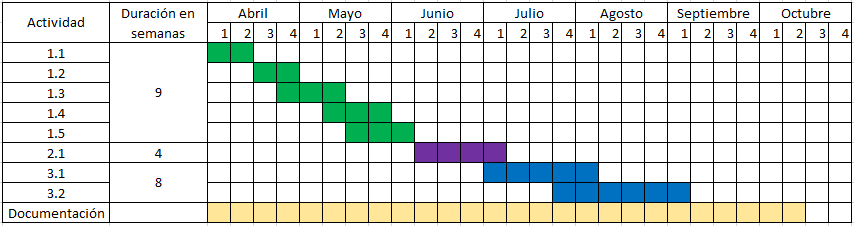
\includegraphics[width=1\linewidth]{Cronograma.PNG}
\label{Cronograma}
\end{figure}

%%%%%%%%%%%%%%%%%%%%%%%%%%%%%%%%%%%%%%%%%%%%%%%%%%%%%%%%%%%%%%%%%%%%%%%%%%%%%%%%%%%%%%%%%%%%%%
\bibliographystyle{abbrv}
\bibliography{BIBLIO.bib}


\section{ Anexos}

Carta de aceptación en el programa de movilidad para el semestre 2020-1.
%%%%%%%%%%%%%%%%%%%%%%%%%%%%%%%%%%%%%%%%%%%%%%%%%%%%%%%%%%%%%%%%%%%%%%%%%%%%%%%%%%%%%%%%%%%%%%

%%%%%%%%%%%%%%%%%%%%%%%%%%%%%%%%%%%%%%%%%%%%%%%%%%%%%%%%%%%%%%%%%%%%%%%%%%%%%%%%%%%%%%%%%%%%%%
\end{document}
